\documentclass[12pt]{beamer}
\usepackage[spanish]{babel}
\usepackage[utf8]{inputenc}
\usepackage{xcolor}
\usepackage{listings}
\usepackage{textcomp}
\usepackage{mathpazo}
\usepackage{courier}
\usepackage{fancyvrb}
\usepackage{amsmath}
\usepackage{url}
\usepackage{hyperref}
\usepackage{enumitem}

\newcommand{\onelinerule}{\rule[2.3ex]{0pt}{0pt}}
\newcommand{\twolinerule}{\rule[6.2ex]{0pt}{0pt}}
\newcommand{\respuesta}{\framebox[\textwidth]{\twolinerule}}
\newcommand{\nombre}{%
  \begin{tikzpicture}[xscale=.4,yscale=.7]
    \draw (0, 0) rectangle (22, 1);
  \end{tikzpicture}%
}
%\newcommand{\rol}   {\framebox[0.3\textwidth]{\onelinerule}}
\newcommand{\rol}{%
  \begin{tikzpicture}[xscale=.4,yscale=.7]
    \draw[gray!40] ( 0, 0) grid      ( 9, 1);
    \draw          ( 0, 0) rectangle ( 9, 1);
    \draw          (10, 0) rectangle (11, 1);
    \draw (9 + .2, .5) -- (10 - .2, .5);
  \end{tikzpicture}%
}
\newcommand{\li}{\lstinline}
\providecommand{\pond}[1]{[{\small\textbf{#1\%}}]}

\lstdefinelanguage{py}{%
  classoffset=0,%
    morekeywords={%
      False,class,finally,is,return,None,continue,for,lambda,try,%
      True,def,from,nonlocal,while,and,del,global,not,with,print,%
      as,elif,if,or,yield,assert,else,import,pass,break,except,in,raise},%
    keywordstyle=\color{black!80}\bfseries,%
  classoffset=1,
    morekeywords={int,float,str,abs,len,raw_input,exit,range,min,max,%
      set,dict,tuple,list,bool,complex,round,sum,all,any,zip,map,filter,%
      sorted,reversed,dir,file,frozenset,open,%
      array,zeros,ones,arange,linspace,eye,diag,dot},
    keywordstyle=\color{black!50}\bfseries,%
  classoffset=0,%
  sensitive=true,%
  morecomment=[l]\#,%
  morestring=[b]',%
  morestring=[b]",%
  stringstyle=\em,%
}

\lstdefinelanguage{testcase}{%
  moredelim=[is][\bfseries]{`}{`},%
  backgroundcolor=\color{gray!20},%
}

\lstdefinelanguage{file}{%
  frame=single,%
}

\lstset{language=py}
\lstset{basicstyle=\ttfamily}
\lstset{columns=fixed}
\lstset{upquote=true}
\lstset{showstringspaces=false}
\lstset{rangeprefix=\#\ }
\lstset{includerangemarker=false}

\newlist{certamen}{enumerate}{1}
\setlist[certamen]{%
  label=\arabic*.,
  font=\LARGE\bfseries,%
  labelindent=-.5in,%
  leftmargin=0pt,%
  labelsep=1em%
}



\usecolortheme{seahorse}
\usefonttheme{serif}

\title{Más sobre interfaces gráficas}
\author{Programación \\ \url{http://progra.usm.cl}}
\date{}

\begin{document}
  \begin{frame}
    \maketitle
  \end{frame}

  \begin{frame}
    \label{repaso-estructura}
    \frametitle{Repaso: estructura de un programa}
    \LARGE
    \lstinputlisting{programas/tkinter/01-ventana.py}
  \end{frame}

  \begin{frame}
    \label{repaso-widgets}
    \frametitle{Repaso: widgets}
    \hfil
    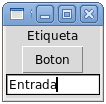
\includegraphics[width=.5\textwidth]{programas/tkinter/capturas/widgets.png}
    \hfil
  \end{frame}

  \begin{frame}
    \label{repaso-crear-widgets}
    \frametitle{Repaso: crear y agregar widgets}
    \begin{columns}[B]
      \column{0.6\textwidth}
        \footnotesize
        \lstinputlisting{programas/tkinter/04-botones.py}
      \column{0.3\textwidth}
        \vfill
        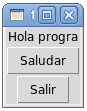
\includegraphics[width=\textwidth]{programas/tkinter/capturas/04.png}
    \end{columns}
  \end{frame}

  \begin{frame}
    \label{estilo}
    \frametitle{Estilo de widgets}
    \begin{columns}[B]
      \column{0.5\textwidth}
        \footnotesize
        \lstinputlisting{programas/tkinter/10-estilo.py}
      \column{0.4\textwidth}
        \vspace{24ex}
        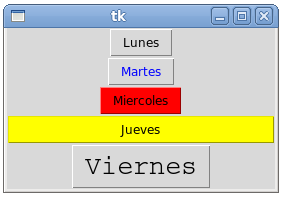
\includegraphics[width=\textwidth]{programas/tkinter/capturas/10.png}
    \end{columns}
  \end{frame}

  \begin{frame}
    \label{configuraciones-estilo}
    \frametitle{Configuraciones de estilo}
    \large
    \begin{tabular}{ll}
      \li!text!   & texto mostrado \\
      \li!width!  & ancho del widget \\
      \li!height! & altura del widget \\
      \li!fg!     & color de las letras (\emph{foreground}) \\
      \li!bg!     & color del fondo (\emph{background}) \\
      \li!font!   & tipo y tamaño de letra \\
      \li!borderwidth! & grosor del borde \\
    \end{tabular}
  \end{frame}

  \begin{frame}
    \label{pack-left}
    \frametitle{Empaquetar hacia el lado}
    \begin{columns}[B]
      \column{0.4\textwidth}
        \footnotesize
        \lstinputlisting{programas/tkinter/11-pack-left.py}
      \column{0.5\textwidth}
        \vspace{24ex}
        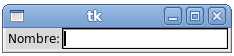
\includegraphics[width=\textwidth]{programas/tkinter/capturas/11.png}
    \end{columns}
  \end{frame}

  \begin{frame}
    \label{grillas}
    \frametitle{Grillas (\li!grid!)}
    \begin{columns}[B]
      \column{0.45\textwidth}
        \footnotesize
        \lstinputlisting{programas/tkinter/12-grid.py}
      \column{0.5\textwidth}
        \vspace{24ex}
        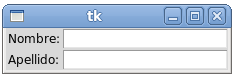
\includegraphics[width=\textwidth]{programas/tkinter/capturas/12.png}
    \end{columns}
  \end{frame}

  \begin{frame}
    \label{ejemplo-marcos}
    \frametitle{Marcos (\li!Frame!)}
    ¿Cómo crear la siguiente interfaz?
    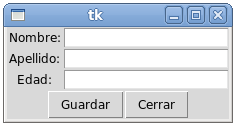
\includegraphics[width=\textwidth]{programas/tkinter/capturas/13.png}

    ¿Ocupamos \li!pack! o \li!grid! para ubicar los widgets?
  \end{frame}


  \begin{frame}
    \label{marcos-0}
    \frametitle{Creación de marcos}
    \begin{center}
      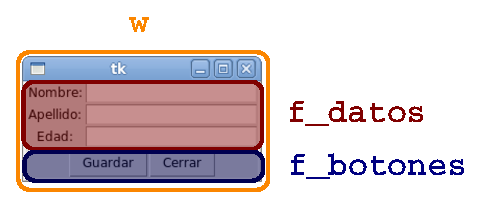
\includegraphics[width=.7\textwidth]{programas/tkinter/capturas/13-0.pdf}
    \end{center}
    \lstinputlisting[linerange=CREAR\ FRAMES-FIN\ CREAR\ FRAMES]
            {programas/tk-frame.py}
    \vfill
  \end{frame}

  \begin{frame}
    \label{marcos-1}
    \frametitle{Widgets del primer marco}
    \begin{center}
      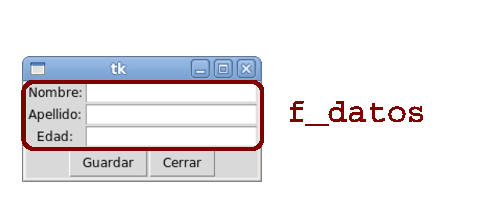
\includegraphics[width=.7\textwidth]{programas/tkinter/capturas/13-1.pdf}
    \end{center}
    \lstinputlisting[linerange=CREAR\ DATOS-FIN\ CREAR\ DATOS]
            {programas/tk-frame.py}
    \vfill
    (y usamos \li!.grid()! para posicionarlos)
  \end{frame}

  \begin{frame}
    \label{marcos-2}
    \frametitle{Widgets del segundo marco}
    \begin{center}
      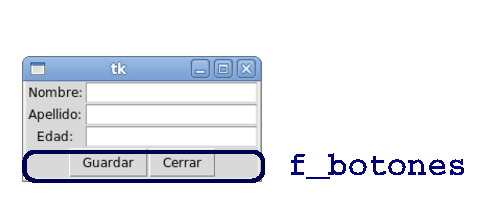
\includegraphics[width=.7\textwidth]{programas/tkinter/capturas/13-2.pdf}
    \end{center}
    \lstinputlisting[linerange=CREAR\ BOTONES-FIN\ CREAR\ BOTONES]
            {programas/tk-frame.py}
    \lstinputlisting[linerange=EMPAQUETADO\ BOTONES-FIN\ EMPAQUETADO\ BOTONES]
            {programas/tk-frame.py}
    \vfill
  \end{frame}

  \begin{frame}
    \label{programa-marcos}
    \frametitle{Programa completo}
    \begin{columns}[B]
      \column{0.45\textwidth}
        \tiny
        \lstinputlisting{programas/tkinter/13-frame.py}
      \column{0.5\textwidth}
        \vspace{24ex}
        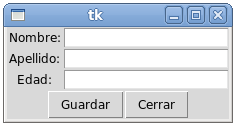
\includegraphics[width=\textwidth]{programas/tkinter/capturas/13.png}
    \end{columns}
  \end{frame}

  \begin{frame}
    \label{ejercicio-edad}
    \frametitle{Ejercicio: calculador de edad}
    \begin{center}
      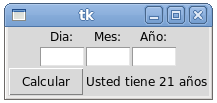
\includegraphics[width=.8\textwidth]{programas/tkinter/capturas/14.png}
    \end{center}
  \end{frame}

  \begin{frame}
    \label{ejercicio-tabla}
    \frametitle{Ejercicio: tabla de multiplicar}
    \begin{center}
      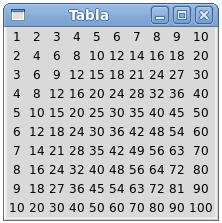
\includegraphics[width=.6\textwidth]{programas/tkinter/capturas/15.png}
    \end{center}
  \end{frame}

  \begin{frame}
    \label{ejercicio-cachipun}
    \frametitle{Ejercicio: cachipún}
    \begin{center}
      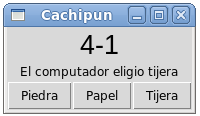
\includegraphics[width=.8\textwidth]{programas/tkinter/capturas/16.png}
    \end{center}
  \end{frame}

\end{document}

